%%%%%%%%%%%%%%%%%%%%%%%%%%%%%%%%%%%%%%%%%%%%%%%%%%%%%%%%%%%%%%%%%%%%%%%%%%%%
%% Author template for Operations Reseacrh (opre) for articles with no e-companion (EC)
%% Mirko Janc, Ph.D., INFORMS, mirko.janc@informs.org
%% ver. 0.95, December 2010
%%%%%%%%%%%%%%%%%%%%%%%%%%%%%%%%%%%%%%%%%%%%%%%%%%%%%%%%%%%%%%%%%%%%%%%%%%%%
%\documentclass[opre,blindrev]{informs3}
\documentclass[opre,nonblindrev]{informs3} % current default for manuscript submission

\OneAndAHalfSpacedXI % current default line spacing
%%\OneAndAHalfSpacedXII
%%\DoubleSpacedXII
%%\DoubleSpacedXI

% If hyperref is used, dvi-to-ps driver of choice must be declared as
%   an additional option to the \documentclass. For example
%\documentclass[dvips,opre]{informs3}      % if dvips is used
%\documentclass[dvipsone,opre]{informs3}   % if dvipsone is used, etc.

%%% OPRE uses endnotes. If you do not use them, put a percent sign before
%%% the \theendnotes command. This template does show how to use them.
\usepackage{endnotes}
\let\footnote=\endnote
\let\enotesize=\normalsize
\def\notesname{Endnotes}%
\def\makeenmark{$^{\theenmark}$}
\def\enoteformat{\rightskip0pt\leftskip0pt\parindent=1.75em
  \leavevmode\llap{\theenmark.\enskip}}

% Private macros here (check that there is no clash with the style)

% Natbib setup for author-year style
\usepackage{natbib}
 \bibpunct[, ]{(}{)}{,}{a}{}{,}%
 \def\bibfont{\small}%
 \def\bibsep{\smallskipamount}%
 \def\bibhang{24pt}%
 \def\newblock{\ }%
 \def\BIBand{and}%

%% Setup of theorem styles. Outcomment only one.
%% Preferred default is the first option.
\TheoremsNumberedThrough     % Preferred (Theorem 1, Lemma 1, Theorem 2)
%\TheoremsNumberedByChapter  % (Theorem 1.1, Lema 1.1, Theorem 1.2)
\ECRepeatTheorems

%% Setup of the equation numbering system. Outcomment only one.
%% Preferred default is the first option.
\EquationsNumberedThrough    % Default: (1), (2), ...
%\EquationsNumberedBySection % (1.1), (1.2), ...

% In the reviewing and copyediting stage enter the manuscript number.
%\MANUSCRIPTNO{} % When the article is logged in and DOI assigned to it,
                 %   this manuscript number is no longer necessary

\usepackage{amsmath}
\usepackage{amssymb}
\usepackage{setspace}
\usepackage{paralist}
\usepackage{graphicx}
\usepackage{url}
\usepackage{algorithm}
\usepackage{algpseudocode}
\usepackage{multicol}
\usepackage{multirow}
\usepackage{csvsimple}

% Frequently used general mathematics
\newcommand{\R}{{\mathbb{R}}}
\newcommand{\Rp}{\R^+}
\newcommand{\Z}{{\mathbb{Z}}}
\newcommand{\Zp}{\Z^+}
\newcommand{\Q}{\mathbb{Q}}
\newcommand{\N}{\mathbb{N}}

% Commands for probability
\renewcommand{\P}{\mathbb{P}}
\newcommand{\E}{\mathbb{E}}
\newcommand{\p}[1]{\P \left[ #1 \right]}
\newcommand{\e}[1]{\E \left[ #1 \right]}
% \newcommand{\ee}[2]{\E_{#1} \left[ #2 \right]}

% Definitions of variables
\newcommand{\X}{X}
\newcommand{\x}{\mathbf{x}}
\newcommand{\xh}{\hat{\x}}
\newcommand{\lh}{\hat{\lambda}}
\newcommand{\mh}{\hat{\mu}}
\newcommand{\xs}{\x^*}
\newcommand{\xit}{\tilde{\mathbf{\xi}}}
\newcommand{\zt}{\tilde{z}}
\newcommand{\zs}{z^*}

% Further variables
\newcommand{\y}{\mathbf{y}}
\renewcommand{\c}{\mathbf{c}}
\newcommand{\A}{\mathbf{A}}
\renewcommand{\b}{\mathbf{b}}
\renewcommand{\k}{\mathbf{k}}
\newcommand{\D}{\mathbf{D}}
\newcommand{\B}{\mathbf{B}}
\renewcommand{\d}{\mathbf{d}}

% Epiconvergence for \plp
\newcommand{\qtrue}{q^{\text{true}}}

% Useful mathematics functions
\newcommand{\keywords}[1]{\par\noindent\enspace\ignorespaces\textbf{Keywords:} #1}
% \newcommand{\keywords}[1]{\par\addvspace\baselineskip\noindent\keywordname\enspace\ignorespaces #1}
% \DeclareMathOperator*{\argmin}{argmin}
% \theoremstyle{plain}
% \newtheorem{theorem}{Theorem}
% \newtheorem{lemma}[theorem]{Lemma}
% \newtheorem{proposition}[theorem]{Proposition}
% \newtheorem{corollary}[theorem]{Corollary}
% 
% \theoremstyle{definition}
% \newtheorem{definition}[theorem]{Definition}
% 
% \theoremstyle{remark}
% \newtheorem{remark}[theorem]{Remark}
\newtheorem{property}{Property}

\newcommand{\st}{\mbox{s.t.}}

% Naming shortcuts
\newcommand{\plp}{$\phi$LP-2}

\bibliographystyle{ormsv080}

%%%%%%%%%%%%%%%%
\begin{document}
%%%%%%%%%%%%%%%%

% Outcomment only when entries are known. Otherwise leave as is and 
%   default values will be used.
%\setcounter{page}{1}
%\VOLUME{00}%
%\NO{0}%
%\MONTH{Xxxxx}% (month or a similar seasonal id)
%\YEAR{0000}% e.g., 2005
%\FIRSTPAGE{000}%
%\LASTPAGE{000}%
%\SHORTYEAR{00}% shortened year (two-digit)
%\ISSUE{0000} %
%\LONGFIRSTPAGE{0001} %
%\DOI{10.1287/xxxx.0000.0000}%

% Author's names for the running heads
% Sample depending on the number of authors;
% \RUNAUTHOR{Jones}
% \RUNAUTHOR{Jones and Wilson}
% \RUNAUTHOR{Jones, Miller, and Wilson}
% \RUNAUTHOR{Jones et al.} % for four or more authors
% Enter authors following the given pattern:
\RUNAUTHOR{Love and Bayraksan}

% Title or shortened title suitable for running heads. Sample:
% \RUNTITLE{Bundling Information Goods of Decreasing Value}
% Enter the (shortened) title:
\RUNTITLE{A Data-Driven Method for Robust Water Allocation under Uncertainty}

% Full title. Sample:
% \TITLE{Bundling Information Goods of Decreasing Value}
% Enter the full title:
\TITLE{A Data-Driven Method for Robust Water Allocation under Uncertainty}

% Block of authors and their affiliations starts here:
% NOTE: Authors with same affiliation, if the order of authors allows, 
%   should be entered in ONE field, separated by a comma. 
%   \EMAIL field can be repeated if more than one author
\ARTICLEAUTHORS{%
\AUTHOR{David Love}
\AFF{University of Arizona, \EMAIL{dlove@email.arizona.edu}, \url{http://math.arizona.edu/~dlove/}}
\AUTHOR{G\"{u}zin~Bayraksan}
\AFF{The Ohio State University, \EMAIL{bayraksan.1@osu.edu}, \url{http://www-iwse.eng.ohio-state.edu/biosketch\_GBayraksan.cfm}}
% Enter all authors
} % end of the block

\ABSTRACT{%
	We investigate the application of techniques from distributionally robust optimization to water allocation in Tucson, AZ under future uncertainty.
	Tucson, like must of the southwestern United States, faces considerable uncertainty in its ability to provide water for its citizens in the future.
	The sources of this uncertainty include (1) the future population growth of the region, (2) the availability of water from the Colorado River, and (3) the effects of climate change and how it relates to water usage.
	This paper presents an approach for integrating forecasts for all these sources of uncertainty in a single optimization model, and provide insight on the value of constructing additional treatment facilities to mitigate the future risks.
}%

% Sample 
%\KEYWORDS{deterministic inventory theory; infinite linear programming duality; 
%  existence of optimal policies; semi-Markov decision process; cyclic schedule}

% Fill in data. If unknown, outcomment the field
\KEYWORDS{Data-driven optimization, water allocation, climate change}
%Optimization under uncertainty, water resources management,  ambiguous stochastic programming, robust optimization, environmental sustainability}
%\HISTORY{}
\maketitle
%%%%%%%%%%%%%%%%%%%%%%%%%%%%%%%%%%%%%%%%%%%%%%%%%%%%%%%%%%%%%%%%%%%%%%

% Samples of sectioning (and labeling) in IJOC
% NOTE: (1) \section and \subsection do NOT end with a period
%       (2) \subsubsection and lower need end punctuation
%       (3) capitalization is as shown (title style).
%
%\section{Introduction.}\label{intro} %%1.
%\subsection{Duality and the Classical EOQ Problem.}\label{class-EOQ} %% 1.1.
%\subsection{Outline.}\label{outline1} %% 1.2.
%\subsubsection{Cyclic Schedules for the General Deterministic SMDP.}
%  \label{cyclic-schedules} %% 1.2.1
%\section{Problem Description.}\label{problemdescription} %% 2.

\section{Introduction and Motivation}

In practice, many optimization problems can be modeled by stochastic programs minimizing the expected value of an uncertain objective function.
However, if the distribution of the uncertain parameters used in the model is incorrect, the stochastic program can give highly suboptimal results.
Such problems have led to the development of distributionally robust optimization, a modeling technique that replaces the probability distribution by a set of distributions, and optimizes the expected cost relative to the worst distribution in the uncertainty set.
One approach that has been recently proposed by \cite{bental2011robust} uses a set of distributions that are sufficiently close in the $\phi$-divergence sense from a given ``nominal'' distribution. 
Of particular interest is the case when the nominal distribution takes the form of the empirical distribution determined by direct observation of data.
In this paper, we adapt the $\phi$-divergence method to the setting of a two-stage stochastic linear program with recourse and call this the two-stage $\phi$-divergence constrained ambiguous stochastic linear program with recourse (\plp).

Using $\phi$-divergences to model ambiguous probability distributions is an attractive approach because it uses the data directly---only those data points or scenarios of interest are used in the calculations.
These scenarios can come from direct observation, results of simulation, or from expert opinion that the decision maker would especially like to be robust against.
Because the \plp\ depends only on these scenarios, the size of the problem is polynomial in the sample size, making the \plp\ computationally tractable.
Furthermore, many $\phi$-divergences are commonly used in statistics (e.g, the $\chi^2$ distance) and provide a natural way of modeling problems under uncertainty. 

\subsection{Related Literature}

In recent years, there has been a growing interest in distributionally robust methods.
Several such studies have focused on solving chance constrained problems in a data-driven setting.
\cite{calafiore2005uncertain} develop a method for generating feasible solutions to data-driven chance constrained problems with high probability, and later \cite{calafiore2006distributionally} develop a method for converting distributionally robust chance constraints into second-order cone constraints.
\cite{erdogan2006ambiguous} study the case where the set of distributions considered is determined by the samples through the Prohorov metric.
\cite{jiang2012data} develop an exact approach to solving several classes of data-driven chance constrained programs, including one defined by the Kullback-Leibler divergence---a type of $\phi$-divergence considered in many further s.

Stochastic programs with uncertain objective functions have long been studied by applying the minimax approach to an expected cost; see, e.g., \cite{zackova1966minimax,dupacova_87}.
Two seminal papers, \cite{shapiro2002minimax} and \cite{shapiro2004class}, developed methods for converting stochastic minimax problems into equivalent stochastic programs with a certain distribution, laying the foundation for a commonly used reformulation technique.

One common method for forming the ambiguity set is moment-based, where all distributions have the same moments (mean, variance, covariance, etc.) are considered.
One early example comes from \cite{scarf1958min}, who provided a distributionally robust model for the newsvendor problem.
More recently, \cite{delage2010distributionally} provide methods for modeling uncertain distributions of a specific form (e.g., Gaussian, exponential, etc.) or using moment-based constraints.

Closer to our case, \cite{pflug2007ambiguity} develop a data-driven method for solving a portfolio selection problem using the Kantorovich distance to define the set of distributions.

\cite{bental2010soft} presents a ``soft'' robust model that allows for changing the level of robustness across the uncertainty set.
Although it is not a distributionally robust stochastic program, this soft robust model, like the distributionally robust models, takes the form of a convex risk measure.

Three recent papers by \cite{wang2010likelihood}, \cite{calafiore2007ambiguous}, and \cite{hukullback} provide similar studies using a specific $\phi$-divergence, described in Section \ref{sec:phi_divergences}, that is defined by the Kullback-Leibler divergence.
Both \cite{wang2010likelihood} and \cite{hukullback} produce dual problems similar to that presented in \cite{bental2011robust} and used here.
\cite{hukullback} differs from this work and the others by considering a continuous distributions, but doesn't relate the nominal distribution to observational data.
Additionally, \cite{klabjan2013robust} uses the $\chi^2$ distance, another $\phi$-divergence, to define an uncertain demand distribution for a stochastic lot-sizing problem using historical data.
Our work unites these previous papers and provides insight into conditions where each $\phi$-divergence should be used and the behavior of the optimization problem as more data is gathered.

\subsection{Contributions}

This paper applies the \plp\ method described in \cite{love2013phi} to a model for water treatment and distribution in a developing region of Tucson, AZ described in \cite{???}.
This work integrates multiple sources of uncertainty into a single optimization model to estimate the relative risk posed by each unknown quantity.
These sources of uncertainty include: (1) population growth in the region considered, (2) Tucson's water allocation from the Colorado River, and (3) the climate of the region and its effect on per-capita demand for water in the region.
We generate scenarios for each of these variables, and integrate them into a single \plp\ stochastic programming model, and estimate the long-run value of constructing additional water treatment facilities to decrease the severity of future water shortages.

\subsection{Organization}

The rest of the paper is organized as follows.
Section \ref{sec:model} presents the water distribution model and the planning scenarios used.
Section \ref{sec:phi_divergences} introduces the $\phi$-divergence, and Section \ref{sec:plp2} presents the $\phi$-divergence model for a two-stage stochastic program with recourse.
Sections \ref{sec:classification} \ref{sec:properties} review our classification of $\phi$-divergences from \cite{love2013phi} and a value-of-data property of the $\phi$-divergence program.
Section \ref{sec:soln_algorithm} presents a decomposition method for solving the \plp\ model.
Section \ref{sec:comp} presents the results of solving the water model with the \plp\ method.
%some of the properties of the \plp\ model.
We end in Section \ref{sec:concl} with our conclusions.



%%%%%%%%%%%%%%%%%%%%%%%%%%%%%%%%%%%%%%%%%%%%%%%%%%%%%%%%%%%%%%%%%%%%%%%%%%%%%%%%
\section{Water Distribution Model}
\label{sec:water}

%% BETTER INTRODUCTION NEEDED!!!!
We applied the \plp method developed here to a problem of water distribution in a currently developing area of Tucson, AZ, shown in Figure \ref{fig:tucson_elevation}.
Tucson is undergoing a period of large population and infrastructure growth, and with that comes an increased demand for water resources.

The majority of Tucson's water comes from the Colorado river, brought in by the Central Arizona Project (CAP), which is indicated by the canal shown in blue in Figure \ref{fig:tucson_elevation}.
This water may then be treated and sent to customers, or pumped underground to one of five aquifers to be saved for future use.
One aquifer recharge facility, the Central Avra Valley Storage And Recovery Project (CAVSARP) is shown in Figure \ref{fig:tucson_elevation}, along with two water treatment plants: the Tucson Water Reclamation Facility and the Haden-Udal Water Treatment Plant.

One southeastern portion of Tucson, outlined in purple in Figure \ref{fig:tucson_elevation}, is being increasingly developed.
This area is split into different elevation zones, shown by the green lines, the demands in each of which will be served by a dedicated pump.
Thus, the green lines also split the region into several pressure zones.
Given the capacity of the existing treatment plants, and the energy cost of pumping the water through a series of pressure zones, Tucson Water is interested in the possibility of building additional treatment facilities  in this area, herein known as the RESIN (Resilient and Sustainable Infrastructures) area.

\begin{figure}
	\FIGURE
	{%
		\includegraphics*[width=.6\textwidth]{tucson_water_images/tucson_elevation.png}%
	}
	{
		A map of Tucson, AZ, showing the RESIN area outlined in purple in the southeastern part.
		The green lines indicate elevation changes, denoting the difference between the pressure zones considered in this study.
		\label{fig:tucson_elevation}
	}
	{}
\end{figure}

A more detailed view of Tucson's water treatment system is shown in Figure \ref{fig:tucson_treatment}.
The blue nodes and arcs indicate the potable water treatment and storage system, which takes CAP water as an input and distributes it to the pressure zones shown in Figure \ref{fig:tucson_zones}.
The purple nodes and arcs indicate non-potable water which can be used to satisfy some (especially agricultural and industrial) demands.
The black nodes indicate waste water that is returned from potable water use.

\begin{figure}
	\FIGURE
	{%
		\includegraphics*[width=.8\textwidth]{tucson_water_images/nodes_central.png}%
	}
	{
		A schematic of the existing water treatment and recharge facilities in Tucson.
		Blue indicated potable water, purple indicates non-potable (reclaimed) water, and black represents waste water.
		\label{fig:tucson_treatment}
	}
	{}
\end{figure}

The pressure zones in the RESIN area, shown in \ref{fig:tucson_zones}, have a largely period structure.
Each pressure zone contains a potable and non-potable demand node.
Note that potable water, being of higher quality, can be used to meet either type of demand.
Each zone also contains a potable-water reservoir and pump, which is used to supply potable to the next pressure zone, and a booster station that provides the conveyance for the non-potable water.
Finally, each zone has a wastewater return, which is transported back to the centralized processing facilities via a gravity flow.

\begin{figure}
	\FIGURE
	{%
		\begin{tabular}{c}
			\includegraphics*[width=.5\textwidth]{tucson_water_images/zones_c_e.png}%
			\includegraphics*[width=.5\textwidth]{tucson_water_images/zones_split.png} \\
			\includegraphics*[width=.6\textwidth]{tucson_water_images/zones_legend.png}
		\end{tabular}
	}
	{
		A schematic illustration of the pressure zones in the RESIN area.
		Each zones contains potable and non-potable demand nodes, a reservoir and booster station for transporting the potable and non-potable water, respectively, and waste water return pipes.
		\label{fig:tucson_zones}
	}
	{}
\end{figure}

Finally, additional infrastructure may be constructed in the form of a satellite wastewater treatment plant (WWTP) may be constructed somewhere in the RESIN area.
Figure \ref{fig:tucson_zones_wwtp} gives an illustration of this using the zone GS.
This satellite WWTP treats wastewater from it's own zone, and higher zones, and supplies additional non-potable water while bypassing the journey all the way back to the centralized treatment facilities shown in Figure \ref{fig:tucson_treatment}.

\begin{figure}
	\FIGURE
	{%
		\begin{tabular}{c}
			\includegraphics*[width=.8\textwidth]{tucson_water_images/zones_south.png}%
		\end{tabular}
	}
	{
		A satellite wastewater treatment plant is shown here, build in pressure zone GS.
		\label{fig:tucson_zones_wwtp}
	}
	{}
\end{figure}

\subsection{Generalized Network Water Model} 
\label{ssec:network_model}

We applied \plp\ to a multi-period generalized network flow model of Colorado River water allocation in Tucson, defined by a set of nodes and directed arcs $(N,\: A)$.
The nodes represent available water supply from the Colorado River, water treatment plants, reservoirs, and water demand sites.
The arcs represent the conveyance system (pipes, etc.) that carry water between the nodes.
Water can be stored in between time periods in reservoirs to meet future demands.
The model aims to find the minimal cost water flows considering energy, treatment, storage, and transportation costs over the planning period. 
Generalized network water allocation models have been used to find water allocations and delivery reliabilities and to assess values of different water use operations; see, e.g., \cite{draper_etal_03}. 

Water flows on arc $(i,j) \in A$ during time period $t = 1, \dots, P$ are represented by decisions $x_{ijt}$.
Each arc $(i,j) \in A$ and time period $t$ has a unit cost $c_{ijt}^x$, loss coefficient $0 \leq a_{ijt} \leq 1$ to account for evaporation, leakage from the pipes, etc., and bounds on the flow $l_{ijt}^x \leq x_{ijt} \leq u_{ijt}^x$.
Each node $j \in N$ has a supply/demand for time period $t$, $b_{jt}$.
Nodes representing reservoirs are able to store water between time periods.
Stored water available at node $j$ at the beginning of time period $t$ is $s_{jt}$, with associated cost $c_{jt}^s$ and bounds $l_{jt}^s \leq s_{jt} \leq u_{jt}^s$.
Finally, water released into the environment from node $j$ in period $t$ is given by $r_{jt}$, with bounds $l_{jt}^r \leq r_{jt} \leq u_{jt}^r$.
The deterministic model is a multi-period generalized network flow model of the form
\begin{align*}
	\min_{x,s,r} \ & \sum_{(i,j) \in A} \sum_{t=1}^P c_{ijt}^x x_{ijt} + \sum_{j \in N} \sum_{t=1}^P c_{jt}^s s_{jt}\\
	\st \ & \sum_{i \in N} x_{jit} + s_{j,t+1} + r_{jt} = \sum_{i \in N} a_{ijt} x_{ijt} + s_{jt} + b_{jt}, \ \ \forall j,t \\
	& l_{ijt}^x \leq x_{ijt} \leq u_{ijt}^x,\ \ \ \forall i,j,t \\
	& l_{jt}^s \leq s_{jt} \leq u_{sjt}^s, \ \ \ \forall j,t \\
	& l_{jt}^r \leq r_{jt} \leq u_{sjt}^r, \ \ \ \forall j,t.
\end{align*}

The model is converted to a two-stage stochastic model with $P_1$ periods in the first stage and $P-P_1$ stages in the second stage.
We assume that the supplies and demands are uncertain, as well as the bounds on the decision variables.
\begin{align}
	\min_{(x,s,r) \in L^1} \ & \sum_{(i,j) \in A} \sum_{t=1}^{P_1} c_{ijt}^x x_{ijt} + \sum_{j \in N} \sum_{t=1}^{P_1} c_{jt}^s s_{jt} + \sum_{\omega=1}^n p_\omega h_\omega(s) \label{eq:gen_network_two_stage} \\
	\st \ & \sum_{i \in N} x_{jit} + s_{j,t+1} + r_{jt} = \sum_{i \in N} a_{ijt} x_{ijt} + s_{jt} + b_{jt},\ \ \ \ \forall j, 1 \leq t \leq P_1, \notag
\end{align}
where the second stage problems
\begin{align}
	h_\omega(s) = \min_{(x,s,r) \in L^2_\omega} \ & \sum_{(i,j) \in A} \sum_{t=P_1+1}^{P} c_{ijt}^x x_{ijt} + \sum_{j \in N} \sum_{t=P_1+1}^{P} c_{jt}^s s_{jt} \label{eq:gen_network_second_stage} \\
	\st \ & \sum_{i \in N} x_{jit} + s_{j,t+1} + r_{jt} = \sum_{i \in N} a_{ijt} x_{ijt} + s_{jt} + b_{jt}^\omega, \ \ \ \ \forall j, P_1+1 \leq t \leq P, \notag
\end{align}
and $L^1$ and $L^2_\omega$ represent the feasible regions defined by the lower and upper variable bounds.

% In the rest of the paper, we simplify the notation for the first-stage (\ref{eq:gen_network_two_stage}) and second-stage (\ref{eq:gen_network_second_stage}) problems as follows.
% In the first stage, decision variables $\{x_{ijt}\}$, $\{s_{jt}\}$ and $\{r_{jt}\}$ become the vector $\x$, costs $\{c_{ijt}^x\}$ and $\{c_{jt}^s\}$ are written as the row vector $\c$, the supply/demand parameters $b_{jt}$ become the vector $\b$ and the constraint matrix is written as $A$.
% In the second stage, we denote the decisions as $\y^\omega$, the costs as $\k^\omega$, the supply/demands as $\d^\omega$, and the constraint matrices multiplying $\y^\omega$ and $\x$ as $D^\omega$ and $B^\omega$, respectively.

% Using the generalized network model (\ref{eq:gen_network_two_stage}) of Colorado River water allocation in the southeastern portion of Tucson, we created a likelihood robust water allocation problem of the form \plp.
% The southeastern portion of Tucson is a newly developing area and is expected to grow considerably.
% The \plp\ water allocation model would help authorities with future water plans in this area while being robust to uncertainties in water supplies and demands.

The model has a total of $P = 41$ time periods, representing years 2010--2050.
%, with projections coming from studies WISP \cite{??} and TAZ \cite{??}.
% We use $P_1 = 10$ time periods for the first stage, and four second-stage scenarios are constructed from high (WISP) and low (TAZ) population estimates along with high and low estimates for the amount of water available for use.
For each time period, the network has 62 nodes representing demand for potable and nonpotable (reclaimed) water, pumps, water treatment plants, and the available water supply from the Colorado River.
The network in each time period has 102 arcs, representing the pipe network carrying the water between the nodes physically and connecting the network to the five reservoirs that connect the time stages in the model.
We use $P_1 = 10$ time periods for the first stage.
Uncertainty in the second stage takes the form of uncertain population (thus, demand for water) and supply of water.
There are a total of 4 scenarios considered in this test instance: (i) high population, high supply, (ii) high population, low supply, (iii) low population, high supply, and (iv) low population, low supply.
Each scenario is assumed to have five observations.
The high population scenarios are more costly as the system needs to meet demand or pay for unmet demand.
The low population scenarios, on the other hand, are not as costly.
We applied the decomposition-based solution algorithm presented in Section \ref{sec:soln_algorithm} to solve this model.

\subsection{Water Demand Regression}
\label{sec:model}

We desire to estimate the weather-dependent demand of water resources in Tucson, and use the results of the climate models to project the future demand for water in the developing area.
To estimate demand separately in each elevation zone, we need a statistical model of the per-capita water demand to be used in conjunction with the zonal population estimates.
For this task, data on monthly demand for water in Tucson from 1991-2011 was obtained from Tucson, along with the recorded amount of rain and the average daily high temperature in each month.

A direct measure of population was only available on a yearly basis, but service counts were available for each month, from which population estimates were inferred in order to estimate the per-capita demand for water.
We performed a linear regression on the total population against the monthly service count data to estimate the population for each month.
The linear regression found that only the number of single family residences was a statistically significant predictor of population size.
The results are shown in Table \ref{tb:population_linear_reg}.
The regression had an adjusted $R^2 = 0.9946$.

\begin{table}
	\TABLE
	{
		Results of the linear regression of population on number of single family units in Tucson Water's service counts.
		\label{tb:population_linear_reg}
	}
	{\begin{tabular}{rrrrr}
		\hline
						   & Estimate  & Std. Error & $t$ value & $p$ \\
		\hline
		(Intercept)    & 2.026e+05 & 7.145e+03  & 28.3 6    & $<2 \cdot 10^{-16}$ \\
		Single Family  & 2.543e+00 & 4.171e-02  & 60.98     & $<2 \cdot 10^{-16}$ \\
		\hline
	\end{tabular}}
	{}
\end{table}

Given the monthly estimates on population, the water demand per capita in gallons per capita per day (GPCD) were calculated for every month in the 1991-2011 data.
A linear regression of these GPCD values on the mean daily high temperature and average precipitation rate for each month, and the year of the observation, was then calculated.
The year of the observation is included because the average GPCD water demand began dropping near the beginning of the 21st century, from over 170 GPCD in 1996 to under 140 GPCD in 2011.
The linear fit, shown in Table \ref{tb:gpcd_linear_reg} has adjusted $R^2 = 0.7266$.

\begin{table}
	\TABLE
	{
		Results of the linear regression of water demand in GPCD on average daily high temperature, precipitation rate, and year.
		\label{tb:gpcd_linear_reg}
	}
	{\begin{tabular}{rrrrr}
		\hline
						   & Estimate  & Std. Error & $t$ value & $p$ \\
		\hline
		(Intercept)    & 2721.2539 & 355.5267   & 7.654     & $4.33\cdot 10^{-13}$ \\
		Temperature    &   3.5830  & 0.1446     & 24.774    & $< 2\cdot 10^{-16}$\\
		Precipitation  &  -2.6329  & 1.1337     & -2.322    & $0.021$ \\
		Year           &  -1.3296  & 0.1776     & -7.486    & $1.24\cdot 10^{-12}$ \\
		\hline
	\end{tabular}}
	{}
\end{table}

This fit, with the year included, projects water demand to be around 145-155 GPCD in 2010, which decreases over time to 100-110 GPCD by 2050.
Tucson Water uses a typical estimate of 120-145 GPCD in their projections.
The range specified by this fit is similar to this for many of the years considered.

A second option for modeling the decrease in water demand as occurring only in a finite span of time.
For this, we choose to regress on a bounded on the value of the year, i.e., choose the value in a set $\{Y_l, Y_l+1, \dots, Y_u\}$ closest to the actual year.
First, the upper bound $Y_u = 2011$ was chosen so that no decrease in water demand would be projected beyond the scope of the data.
The value $Y_l = 2004$ was then selected to generate the best fit to the data.
This piecewise fit is shown in Table \ref{tb:gpcd_piecewise_reg}, and has $R^2 = 0.7634$.

\begin{table}
	\TABLE
	{
		Results of the linear regression of water demand in GPCD on average daily high temperature, precipitation rate, and and the bounded year.
		\label{tb:gpcd_piecewise_reg}
	}
	{\begin{tabular}{rrrrr}
		\hline
						   & Estimate  & Std. Error & $t$ value & $p$ \\
		\hline
		(Intercept)    & 9254.0201 & 904.3062   & 10.233    & $<2\cdot 10^{-16}$ \\
		Temperature    & 3.5913    & 0.1345     & 26.694    & $<2\cdot 10^{-16}$ \\
		Precipitation  & -2.2570   & 1.0510     & -2.148    & $0.0327$ \\
		Bounded Year   & -4.5847   & 0.4509     & -10.167   & $<2\cdot 10^{-16}$ \\
		\hline
	\end{tabular}}
	{}
\end{table}

The piecewise fit typically predicts demands of 135-145 GPCD throughout the 2010-2050 time period, in line with Tucson Water's predictions.

\subsection{Population \& Water Supply Estimates}

\begin{table}
	\TABLE
	{
		Population estimates for the RESIN area.
		\label{tb:population}
	}
	{\begin{tabular}{lcc}
		\hline
		         & \multicolumn{2}{c}{population} \\
		Estimate & 2010 & 2050 \\
		\hline
		\cite{taz}    &  53,028 &   460,000 \\
		\cite{wisp}   &  53,028 &   740,000 \\
		\cite{tucson} & 750,000 & 1,300,000 \\
		\hline
	\end{tabular}}
	{}
\end{table}

Estimates of the population in each pressure zone were compiled from two population studies in Pima County in Arizona: the Water \& Wastewater Infrastructure, Supply \& Planning Study \citep{wisp} and the Traffic Analysis Zone (TAZ) \citep{taz}.
\cite{taz} provides a lower estimate of growth in the RESIN area, while \cite{wisp} provides the higher estimate.
The RESIN area represents a subset of the population served by Tucson Water, the population of which is estimated from \cite{tucson}.
Sample values can be seen in Table \ref{tb:population}.

Tucson Water has a yearly CAP water allocation of 144,000 acre-feet, which may be reduced in the event of an extended drought reducing the flows of the Colorado river.
The Arizona Department of Water Resources believes that a 10\% reduction to 130,000 acre-feet is the maximum realistic reduction by 2050 \cite{scott2012scenario}, which is used in this study.
The water allocation to the RESIN area is determined by the proportion of the Tucson Water service population in the RESIN area.
I.e., under the \cite{wisp} growth scenario with the full CAP allocation, the RESIN area is allocated about 81,970 acre-feet in 2050.

\subsection{Climate Models Used}

A list of the climate models used in this paper is shown in Table \ref{tb:climate_models}.
Bias-Corrected and Spatially Downscaled (BCSD) data from Coupled Model Intercomparison Project: Phase 5 (CMIP5) was obtained from \cite{cmip5}.
Additional information on the downscaled data can be found in \cite{bcsdreclamation}.
Each model included predictions of the variables \texttt{tasmax} and \texttt{pr}, the average daily high temperature ($^\circ C$) and the average precipitation rate (mm/day) in each month.

\begin{table}
	\TABLE
	{
		A list of climate models used in this analysis
		\label{tb:climate_models}
	}
	{\begin{tabular}{p{.7\textwidth}|r}
		\hline
		Institution & Model \\
		\hline
		\hline
		Commonwealth Scientific and Industrial Research Organization (CSIRO) and Bureau of Meteorology (BOM), Australia & CSIRO-mk-3-6-0 \\
		\hline
		\multirow{2}{*}{Geophysical Fluid Dynamics Laboratory} & GFDL-CM3 \\
		 & GFDL-ESM2M \\
		\hline
		Met Office Hadley Centre & HadGEM2-ES \\
		\hline
		\multirow{3}{*}{\vbox{Atmosphere and Ocean Research Institute (The University of Tokyo), National Institute for Environmental Studies, and Japan Agency for Marine-Earth Science and Technology}}  & MIROC5 \\
		 & MIROC-ESM \\
		 & \\
		\hline
	\end{tabular}}
	{}
\end{table}

Each model had output associated with a given path for future emissions.
Our analysis includes two paths: RCP8.5 and RCP4.5.
The former is the high emissions scenario which ultimately results in increased warming in the long term.
The latter scenario is a lower emissions scenario, in which emissions stabilize before 2100.
A comparison of the model output of the average daily high temperature for 2040-2050 for emissions path RCP8.5 is shown in Table \ref{tb:model_comparison_temperature}.

\begin{table}
	\TABLE
	{
		A comparison of projected ($\geq 2040$) average daily high temperatures ($^\circ C$) with the historical record (1991-2011) in Tucson, AZ.
		All values come from models using emissions path RCP8.5.
		\label{tb:model_comparison_temperature}
	}
	{\csvautotabular{tables/temperature.csv}}
	{}
\end{table}

%%%%%%%%%%%%%%%%%%%%%%%%%%%%%%%%%%%%%%%%%%%%%%%%%%%%%%%%%%%%%%%%%%%%%%%%%%%%%%%%
\section{Introduction to $\phi$-Divergences}
\label{sec:phi_divergences}

In this section we define the concept of a $\phi$-divergence, and describe some of the properties that will be used through the remainder of the paper.
\cite{pardo2005statistical} provides a good overview of much of the known properties of $\phi$-divergences.
Many results in this section can be also found in \citep{bental2011robust}.

$\phi$-divergences are used in statistics to measure the ``distance'' between two distributions. 
In the discrete case, $\phi$-divergences can be used generally to measure the distance between two non-negative vectors $p = (p_1, \dots, p_n)^T$ and $q = (q_1, \dots, q_n)^T$, and specifically when $p$ and $q$ are probability vectors; i.e., satisfying $\sum_{\omega=1}^n p_\omega = \sum_{\omega=1}^n q_\omega = 1$.
The $\phi$-divergence is defined by
\[
	I_\phi(p,q) = \sum_{\omega=1}^n q_\omega \phi\left(\frac{p_\omega}{q_\omega}\right),
\]
where $\phi(t)$, called the $\phi$-divergence function, is a convex function on $t \geq 0$ such that $\phi(1) = 0$, and with the additional interpretations that $0 \phi(a/0) = a \lim_{t \rightarrow \infty} \frac{\phi(t)}{t}$, and $0 \phi(0/0) = 0$.
If both $p$ and $q$ are probability vectors, as we assume throughout this paper, we can additionally assume without loss of generality that $\phi(t) \geq 0$.
The function $\phi(t)$ can be modified as $\psi(t) = \phi(t) + c(t-1)$ with an appropriately chosen constant $c$ such that $\psi(t) \geq 0$ for all $t$, and $I_\psi(p,q) = I_\phi(p,q)$ for all probability vectors $p,q$.
If $\phi(t)$ is differentiable at $t = 1$ this can be done by selecting $c = -\phi'(1)$.
%; see, e.g., the Likelihood divergence and Burg entropy in Table~\ref{tb:phi_definitions}.

$\phi$-divergences are not, in general, metrics.
For example, most $\phi$-divergences do not satisfy the triangle inequality and many are not symmetric in the sense that $I_\phi(p,q) \neq I_\phi(q,p)$.
One exception is the Variation distance, which is equivalent to the $L^1$-distance between the vectors.

A $\phi$-divergence has an adjoint, defined by
\begin{equation} \label{eq:adjoint}
	\tilde{\phi}(t) = t \phi\left(\frac{1}{t}\right),
\end{equation}
which satisfies all criteria for a $\phi$-divergence \citep{bental1991certainty}, and has the property that $I_{\tilde{\phi}}(p,q) = I_\phi(q,p)$.
Divergences that are symmetric with respect to the input vectors are known as self-adjoint.

The problem formulation involves use of the conjugate $\phi^* : \R \rightarrow \R \cup \{\infty\}$, defined as
\begin{equation} \label{eq:conjugate}
	\phi^*(s) = \sup_{t \geq 0} \{st - \phi(t)\}.
\end{equation}
The conjugate $\phi^*$ is a nondecreasing convex function and may be undefined above some upper bound $\bar{s}$.

Table \ref{tb:phi_definitions} lists some common examples of $\phi$-divergences, along with their adjoints and conjugates.
For all divergences, $\phi(t) = \infty$ for $t < 0$, and the value of the conjugate is listed only in its domain; i.e., $\{s : \phi^*(s) < \infty\}$.
Most of these common divergences are widely used in statistics and information theory.\
Table \ref{tb:phi_definitions} also lists a divergence, labeled ``Likelihood,'' that is somewhat different from the others.
The Likelihood divergence is equivalent to the Burg entropy when comparing probability vectors, but does not satisfy the normalizing condition $\phi(t) \geq 0$.
This divergence is included because \cite{wang2010likelihood} use it to formulate a distributionally robust newsvendor problem so that the ambiguity set of distributions have a sufficiently high empirical likelihood. 
They refer to this as the Likelihood Robust Optimization.
We also note that \cite{calafiore2007ambiguous}, \cite{hukullback}, and \cite{wang2010likelihood} all use a different naming convention than the one given here, referring to the Likelihood divergence or Burg entropy as the ``Kullback-Leibler (KL) divergence''---reversing the order of the arguments $p$ and $q$ relative to the notation presented here.
In this paper, $q$ denotes the nominal distribution.

\begin{table}
	\TABLE
	{
		Definitions of some common $\phi$-divergences, along with their adjoints $\tilde{\phi}(t)$ and conjugates $\phi^*(s)$
		\label{tb:phi_definitions}
	}
	{\begin{tabular}{lccccc}
		\hline \\
		Divergence                        & $\phi(t)$          & $\tilde{\phi}(t)$               & $\phi(t), t \geq 0$   & $I_\phi(p,q)$     & $\phi^*(s)$ \\
		\hline
		Kullback-Leibler                 & $\phi_{kl}$        & $\phi_b$                        & $t\log t - t + 1$     & $\sum p_\omega \log\left(\frac{p_\omega}{q_\omega}\right)$ & $e^s - 1$ \\
		Burg Entropy                      & $\phi_b$           & $\phi_{kl}$                     & $-\log t + t - 1$     & $\sum q_\omega \log\left(\frac{q_\omega}{p_\omega}\right)$ & $-\log(1-s),\ s < 1$  \\
		J-Divergence                      & $\phi_j$           & $\phi_j$                        & $(t-1)\log t$         & $\sum (p_\omega - q_\omega) \log\left(\frac{p_\omega}{q_\omega}\right)$ & No closed form \\
		Likelihood                        & $\phi_l$           & $t\log t $                      & $-\log t$             & $\sum q_\omega \log\left(\frac{q_\omega}{p_\omega}\right)$ & $-\log(-s) - 1,\ s < 0$ \\
		$\chi^2$-Distance                 & $\phi_{\chi^2}$    & $\phi_{m\chi^2}$                & $\frac{1}{t} (t-1)^2$ & $\sum \frac{(p_\omega-q_\omega)^2}{p_\omega}$              & $2 - 2\sqrt{1-s},\ s < 1$  \\
		Modified $\chi^2$-Dist.           & $\phi_{m\chi^2}$   & $\phi_{\chi^2}$                 & $(t-1)^2$             & $\sum \frac{(p_\omega - q_\omega)^2}{q_\omega}$            & $\begin{cases} -1 & s < -2 \\ s + \frac{s^2}{4} & s \geq -2 \end{cases}$ \\
% 		$\chi$-div,  $\theta > 1$ & $\phi_\chi^\theta$ & $t^{1-\theta}\phi_\chi^\theta$ & $|t-1|^\theta$         & $\sum q_\omega |1-\frac{p_\omega}{q_\omega}|^\theta$       & $\begin{cases} -1 & s \leq -\theta \\ s + (\theta-1)\left(\frac{|s|}{\theta}\right)^\frac{\theta}{\theta-1}  & s \geq -\theta \end{cases}$ \\
		Variation Distance                & $\phi_v$           & $\phi_v$                        & $|t-1|$               & $\sum |p_\omega - q_\omega|$                               & $\begin{cases} -1 & s \leq -1 \\ s & -1 \leq s \leq 1 \end{cases}$ \\
		Hellinger Distance                & $\phi_h$           & $\phi_h$                        & $(\sqrt{t} - 1)^2$    & $\sum (\sqrt{p_\omega} - \sqrt{q_\omega})^2$               & $\frac{s}{1-s},\ s < 1$ \\
	\hline
	\end{tabular}}
	{}
\end{table}

%%%%%%%%%%%%%%%%%%%%%%%%%%%%%%%%%%%%%%%%%%%%%%%%%%%%%%%%%%%%%%%%%%%%%%%%%%%%%%%%
\section{$\phi$-Divergence Constrained Ambiguous Stochastic Program}
\label{sec:plp2}

In this section we provide primal and dual formulations and basic properties of two-stage ambiguous stochastic linear programs constructed via $\phi$-divergences.

%%%%%%%%%%%%%%%%%%%%%%%%%%%%%%%%%%%%%%%%%%%%%%%%%%%%%%%%%%%%%%%%%
\subsection{Formulation}
\label{ssec:form}

We begin with a two-stage stochastic linear program with recourse (SLP-2).
Let $\x$ be a vector of first-stage decision variables with cost vector $\c$, constraint matrix $\A$ and right-hand side $\b$.
We assume a finite distribution given by $q_\omega$ with scenarios indexed by $\omega = 1, \dots, n$.
The SLP-2 is
\begin{align}
	\min_\x \ & \left\{ \c\x + \sum_{\omega=1}^n q_\omega h_\omega(\x) : \A\x = \b, \x \geq 0 \right\}, \label{eq:slp_first_stage}% \\
% 	\st \ & \A\x = \b \nonumber  \\
% 	&\ \ \ \x \geq 0 \nonumber
\end{align}
where
\begin{align}
	h_\omega(\x) = \min_{\y^\omega} \ & \left\{ \k^\omega \y^\omega : \D^\omega \y^\omega = \B^\omega \x + \d^\omega, \y^\omega \geq 0 \right\}. \label{eq:slp_second_stage}
\end{align}
We assume relatively complete recourse; i.e., the second-stage problems $h_\omega(\x)$ are feasible for every feasible solution $\x$ of the first-stage problem; and that the second-stage problems $h_\omega(\x)$ are dual feasible for every feasible solution $\x$ of the first-stage problem.
For convenience, we denote $X = \{\x : \A\x = \b, \x \geq 0\}$.

The SLP-2 formulation assumes that the distribution $\{q_\omega\}_{\omega=1}^n$ is known.
However, in many applications the distribution is itself unknown.
One technique to deal with this is to replace the known distribution with an {\it ambiguity set} of distributions; i.e., a set of distributions that is believed to contain the true distribution.
In this paper, we construct the ambiguity set by considering all distributions whose $\phi$-divergence from the nominal distribution $q$ is sufficiently small.
Throughout portions of this paper, we focus on a data-driven setting and assume that $q$ is generated from observations, where scenario $\omega$ has been observed $N_\omega$ times, with $N = \sum_{\omega=1}^n N_\omega$ total observations, although $q$ can be obtained in other ways.
In SLP-2, this data-driven setting would correspond to the probability of scenario $\omega$ to be $q_\omega = \frac{N_\omega}{N}$.

By replacing the specific distribution in SLP-2 with a set of distributions sufficiently close to the nominal distribution with respect to $\phi$-divergence, we create the \plp\ model.
In the \plp, the objective function is minimized with respect to the worst-case distribution selected from the ambiguity set of distributions.
The resulting minimax formulation of \plp\ is
\begin{equation}
	\min_{\x \in X} \max_{p \in \mathcal{P}} \left\{ \c\x + \sum_{\omega=1}^{n} p_\omega h_\omega(\x) \right\}, \label{eq:plp_primal}
\end{equation}
where the ambiguity set is
\begin{align}
	\mathcal{P} = & \left\{ \sum_{\omega = 1}^{n} q_\omega \phi\left(\frac{p_\omega}{q_\omega}\right) \leq \rho, \right. \label{eq:plp_primal_divergence} \\
	& \ \sum_{\omega=1}^{n} p_\omega = 1, \label{eq:plp_primal_probability} \\
	& \ \left. p_\omega \geq 0,\ \forall \omega \right\}. \label{eq:nonneg}
\end{align}
We refer to (\ref{eq:plp_primal_divergence}) as the $\phi$-divergence constraint and (\ref{eq:plp_primal_probability}) and (\ref{eq:nonneg}) simply ensure a probability measure.
We discus how to determine $\rho$ in (\ref{eq:plp_primal_divergence}) in Section \ref{ssec:robust_level}.

Taking the dual of the inner maximization problem, with dual variables $\lambda$ and $\mu$, of constraints (\ref{eq:plp_primal_divergence}) and (\ref{eq:plp_primal_probability}), respectively, and combining the two minimizations gives \plp\ in dual form
\begin{align}
	\min_{\x,\lambda,\mu} \ & \c\x + \mu + \rho \lambda + \lambda \sum_{\omega=1}^{n} q_\omega \phi^*\left(\frac{h_\omega(\x) - \mu}{\lambda}\right) \label{eq:plp_two_stage} \\
	\st \ & \x \in X \nonumber \\
	& \frac{h_\omega(\x) - \mu}{\lambda} \leq \lim_{t \rightarrow \infty} \frac{\phi(t)}{t}, \ \forall \omega \label{eq:plp_feas_constraint}\\
	& \lambda \geq 0, \nonumber
\end{align}
where $h_\omega(\x)$ and the second-stage problems are as given in (\ref{eq:slp_second_stage}), $0\phi^*(s/0)=0$ if $s\leq 0$ and  $0\phi^*(s/0)=+\infty$ if $s > 0$.
Note that some $\phi$, such as the J-Divergence, have no closed form representation of $\phi^*$, but can be expressed as the sum of other divergences---Burg Entropy and KL divergence---which allows the dual to be formed; see \citep{bental2011robust} for details.
Theorem 1 of \cite{bental2011robust} contains a derivation of the dual problem.
Note in particular that the dual formulation is accurate even for $q_\omega = 0$ for some $\omega$.
Also note that the right-hand side of (\ref{eq:plp_feas_constraint}) contains a limit.
For some $\phi$-divergences, like the KL divergence, this limit is $\infty$, in which case (\ref{eq:plp_feas_constraint}) is redundant.
However, other $\phi$-divergences, like the Hellinger distance, have a finite limit, inducing this constraint.
Throughout the paper, we use $s_\omega$ to denote
\begin{equation}
	s_\omega = \frac{h_\omega(\x) - \mu}{\lambda}. \label{eq:s_omega_definition}
\end{equation}


%%%%%%%%%%%%%%%%%%%%%%%%%%%%%%%%%%%%%%%%%%%%%%%%%%%%%%%%%%%%%%%%%
\subsection{Basic Properties}
\label{ssec:basicprop}

In this section we list some basic properties of \plp.
Most of these have already been noted earlier (e.g., by \cite{bental2011robust} and others for specific $\phi$-divergences) but we list them for completeness.
Some of these properties help with our specialized solution method and we refer to them in later sections.

\begin{property}
	\label{property:convex}
	\plp\ is a convex program.
\end{property}

\begin{property}
	\label{property:coherent_risk_measure}
	\plp\ is equivalent to minimizing a coherent risk measure.
\end{property}

Note that being a coherent risk measure implies that \plp\ is a convex problem.
The convexity of LRO was also noted in \cite{wang2010likelihood}.

\begin{property}
	\label{property:time_structure}
	\plp\ preserves the time structure of SLP-2.
\end{property}

\begin{property}
	\label{property:primal_dual_relation}
	The worst-case distribution can be calculated with the equations
	\begin{equation}\label{eq:p_worst}
		\frac{p_\omega}{q_\omega} \in \partial \phi^*\left(s_\omega\right), \ \ \ \ \ \sum_{\omega=1}^n q_\omega \phi\left(\frac{p_\omega}{q_\omega}\right) \leq \rho, \ \ \ \ \ \sum_{\omega=1}^n p_\omega = 1.
	\end{equation}
\end{property}

We now discuss these properties. A coherent risk measure is defined in \citep{rockafellar2007coherent}, which shows that minimizing a coherent risk measure over a polyhedron implies that \plp\ is a convex problem.
The convexity of \plp\ was also noted in \citep{bental2011robust}.
Properties \ref{property:time_structure} and \ref{property:primal_dual_relation} help with our decomposition-based solution method described in Section \ref{sec:soln_algorithm}. 
The preservation of time structure, as can be seen in (\ref{eq:plp_two_stage}), allows us to decompose the problem and convert (sub-)derivatives of $h_\omega(\x)$ to (sub-)derivatives of $\phi^*\left(s_\omega\right)$, aiding in our decomposition-based solution method. 
The appearance of the conjugate $\phi^*(s)$ in the objective of (\ref{eq:plp_two_stage}) gives a method for retrieving the worst-case distribution from the dual problem, as detailed in Property \ref{property:primal_dual_relation}.
In many cases, the first equation in (\ref{eq:p_worst}) is sufficient to calculate $\{p_\omega\}_{\omega=1}^n$.
In addition, $\phi^*$ is often differentiable and so we have the relationship $p_\omega = q_\omega \phi^{* \prime}(s_\omega)$.
Special cases when $\lambda = 0$ or $q_\omega = 0$ for some $\omega$ are detailed in Section \ref{sec:classification}.



%%%%%%%%%%%%%%%%%%%%%%%%%%%%%%%%%%%%%%%%%%%%%%%%%%%%%%%%%%%%%%%%%
\subsection{The Level of Robustness}
\label{ssec:robust_level}

The literature on $\phi$-divergences provides some insight on choosing a reasonable asymptotic value of $\rho$ in the data-driven setting. 
When $\phi$ is twice continuously differentiable around $1$ with $\phi^{\prime \prime}(1)>0$, Theorem 3.1 of \cite{pardo2005statistical} shows that the statistic $T^\phi_N(q^N,\qtrue) = \frac{2N}{\phi''(1)} \sum_{\omega=1}^n \qtrue_\omega \phi\left(\frac{q^N_\omega}{\qtrue_\omega}\right)$ converges in distribution to a $\chi^2$-distribution with $n-1$ degrees of freedom, where $q^N$ denotes the empirical distribution ($q^N_\omega = N_\omega/N$), and $\qtrue$ denotes the underlying true distribution.
Most $\phi$-divergences in Table~\ref{tb:phi_definitions} satisfy this differentiability condition.
\cite{bental2011robust} then use this result to suggest the asymptotic value
\begin{equation} \label{eq:asymptotic_rho}
	\rho = \frac{\phi''(1)}{2N} \chi^2_{n-1,1-\alpha},
\end{equation}
where $\chi^2_{n-1,1-\alpha}$ is the $1-\alpha$ percentile of a $\chi^2_{n-1}$ distribution, which produces an approximate $1-\alpha$ confidence region on the true distribution.
For corrections for small sample sizes and more details, we refer the readers to \citep{pardo2005statistical} and \citep{bental2011robust}. 

We are now ready to present the main contributions of this paper.

%%%%%%%%%%%%%%%%%%%%%%%%%%%%%%%%%%%%%%%%%%%%%%%%%%%%%%%%%%%%%%%%%%%%%%%%%%%%%%%%
\section{A Classification of $\phi$-Divergences}
\label{sec:classification}

Given that there are many $\phi$-divergences to choose from, it is important to study how $\phi$-divergences act within an ambiguous (or, distributionally robust) stochastic optimization model. 
We present a classification of $\phi$-divergences into four types, resulting from an examination of the limiting behavior of $\phi(t)$ as $t \rightarrow 0$ and $t \rightarrow \infty$.
Different classifications may be suitable to different problem types and desired qualities in the ambiguous model---we discuss modeling considerations with respect to our classification in Section \ref{ssec:modeling}.

%%%%%%%%%%%%%%%%%%%%%%%%%%%%%%%%%%%%%%%%%%%%%%%%%%%%%%%%%%%%%%%
\subsection{Suppressing and Popping of Scenarios}
\label{ssec:suppressandpop}

As motivation for our classification, consider a self-adjoint $\phi$-divergence, which satisfies the relation
\begin{equation} \label{eq:self_adjoint_classification}
	\frac{\phi(t)}{t} = \phi\left(\frac{1}{t}\right),
\end{equation}
and consider $t \rightarrow \infty$.
If both sides of (\ref{eq:self_adjoint_classification}) are finite in the limit, then we see a correspondence between the boundedness of $\phi(t)$ for $t < 1$ and linear growth of $\phi(t)$ for $t > 1$.
On the other hand, infinite limits of (\ref{eq:self_adjoint_classification}) indicate a correspondence between superlinear growth of $\phi(t)$ for $t > 1$ and unboundedness of $\phi(t)$ for $t < 1$.

Recall the definition of the ambiguity set, in particular, the $\phi$-divergence constraint (\ref{eq:plp_primal_divergence}). 
In the \plp, $\phi$ has arguments given by ratios of probabilities, $\tfrac{p_\omega}{q_\omega}$ and the limits $t \rightarrow 0$ and $t \rightarrow \infty$ correspond to the cases when $p_\omega = 0$ and $q_\omega = 0$, respectively.
Consider each of these limiting cases:
\begin{itemize}
	\item {\sc Case 1:} $q_\omega > 0$ but $p_\omega = 0$.
		We call this the ``{\bf Suppress}'' behavior because a scenario with a positive probability in the nominal distribution can take zero probability in the ambiguous problem. In this case we need to examine $\lim_{t \searrow 0} \phi(t)$:
	\begin{itemize}
		\item If $\lim_{t \searrow 0} \phi(t) = \infty$, the ambiguity region will never contain distributions with $p_\omega = 0$ but $q_\omega > 0$.
		\item On the other hand, if $\lim_{t \searrow 0} \phi(t) < \infty$, the ambiguity region could contain such a distribution, provided $q_\omega$ is sufficiently small or $\rho$ is sufficiently large.
			We say that such a $\phi$-divergence can \emph{suppress} scenario $\omega$.
	\end{itemize}
	\item {\sc Case 2:} $q_\omega = 0$ but $p_\omega > 0$.
		We call this the ``{\bf Pop}'' behavior because a scenario with zero probability in the nominal distribution can have a positive probability (or, pop) in the ambiguous problem. In this case, we need to examine $\lim_{t \nearrow 0} \frac{\phi(t)}{t}$:
	\begin{itemize}
		\item If $\lim_{t \nearrow 0} \frac{\phi(t)}{t} = \infty$, the ambiguity region can never contain distributions with $p_\omega > 0$ but $q_\omega = 0$.
		\item On the other hand, if $\lim_{t \nearrow 0} \frac{\phi(t)}{t} < \infty$, the ambiguity region will admit sufficiently small $p_\omega$.
			We say that these $\phi$-divergences can \emph{pop} scenario $\omega$.
	\end{itemize}
	\item {\sc Case 3:} $p_\omega = 0$ but $q_\omega = 0$.
		Such a situation has no contribution to the divergence, since $0 \phi\left(\tfrac{0}{0}\right) = 0$.
\end{itemize}

\noindent These two limiting cases describing suppressing and popping behavior in $\phi$-divergences create four distinct categories.
Examples of divergences in each category are given in Table \ref{tb:phi_categories}.
Note that $\phi$ can suppress scenarios if and only if its adjoint $\tilde{\phi}$ can pop scenarios, and vice versa.
This means that self-adjoint $\phi$-divergences are either capable of both popping and suppressing scenarios or capable of neither.

\begin{table}
	\TABLE
	{
		Examples of $\phi$-divergences fitting into each category.
		The number in parentheses under the ``Can Suppress Scenarios'' column denotes the subcategory detailed in \cite{love2013phi}.
		\label{tb:phi_categories}
	}
	{\begin{tabular}{l|p{.33\textwidth}p{.33\textwidth}}
		 & Can Suppress Scenarios & Cannot Suppress Scenarios \\
		 \hline
		 Can Pop Scenarios %
			& \parbox{.33\textwidth}{Hellinger Distance (2),\\Variation Distance (1)} %
			& \parbox{.33\textwidth}{Burg Entropy,\\$\chi^2$-Distance} \smallskip \\
		 Cannot Pop Scenarios %
			& \parbox{.33\textwidth}{Kullback-Leibler Divergence (2),\\Modified $\chi^2$-Distance (1)} %
			& \parbox{.33\textwidth}{J-Divergence}
	\end{tabular}}
	{}
\end{table}

%%%%%%%%%%%%%%%%%%%%%%%%%%%%%%%%%%%%%%%%%%%%%%%%%%%%%%%%%%%%%%%
\subsection{Modeling Considerations When Choosing a Divergence}
\label{ssec:modeling}

We offer the following suggestions for choosing an appropriate $\phi$-divergence classification for the data available.
First, consider whether to choose a distribution that can suppress scenarios.
If the problem scenarios come from high-quality observed data, one may wish to avoid divergences that can suppress scenarios.
However, if the data is poorly sampled or comes from opinion rather than observation or simulation, the option of suppressing scenarios may result in a solution with better robustness properties.

Next, consider whether to choose a distribution that allows for popping scenarios.
If the problem scenarios come strictly from observation, with little theoretical understanding of the problem, we suggest choosing a divergence that cannot pop scenarios.
However, if the problem scenarios come from a mix of observed/simulated data and expert opinion about scenarios of interest, then divergences that can pop present an interesting modeling choice.
This allows for including interesting but unobserved scenarios, allowing the mathematical program to assign an appropriate probability to them.



%%%%%%%%%%%%%%%%%%%%%%%%%%%%%%%%%%%%%%%%%%%%%%%%%%%%%%%%%%%%%%%%%%%%%%%%%%%%%%%%
\section{Data-Driven Considerations}
\label{sec:properties}

In this section we assume the nominal distribution $q$ is the empirical distribution ($q_\omega = \tfrac{N_\omega}{N}$) and provide insight into how the \plp\ changes when a single observation in Section \ref{ssec:value}.
This analysis must consider how $\rho$ changes as additional samples are taken; therefore, we use $\rho_N$ to emphasize the dependence on sample size in this section.
To be consistent with the known $\phi$-divergence results stated in Section \ref{ssec:robust_level}, we assume $\rho_N = \frac{\rho_0}{N}$.

\subsection{The Value of Data} \label{ssec:value}

With a data-driven formulation such as \plp, it is natural to ask how the optimal value and solution changes as more data is gathered.
In particular, one might be concerned about being overly conservative in the problem formulation and thus missing the opportunity to find a better solution to the true distribution.
For \plp, this means that the initial model is likely to be more conservative in an effort to be robust, while the new information could make the model less conservative because new information removes the current worst-case distribution from the ambiguity set.  
Below, we present a simple method of determining if taking an additional sample will eliminate the old worst-case distribution and allow for better optimization; i.e., a lower-cost solution.
%We also provide a way of estimating the probability of sampling such an observation.

\begin{theorem}
	\label{thm:value}
	An additional sample of scenario $\hat{\omega}$ will result in a decrease in the worst-case expected cost of the \plp\ if the following condition is satisfied
	\begin{equation} \label{eq:cost_decrease_cond}
		\sum_{\omega=1}^n q_\omega \phi^{*\prime}\left(\frac{N}{N+1}s^*_\omega\right) \left(\frac{N}{N+1}s^*_\omega\right) > \phi^*\left(\frac{N}{N+1}s^*_{\hat{\omega}}\right),
	\end{equation}
	where $s^*_\omega = \dfrac{h_\omega(\x^*_N) - \mu^*_N}{\lambda^*_N}$ and $(\x^*_N,\mu^*_N,\lambda^*_N)$ solve the $N$-sample problem with $q_\omega = \tfrac{N_\omega}{N}$.
\end{theorem}

We can interpret \eqref{eq:cost_decrease_cond} as follows. If an additional sample is taken from the unknown distribution and the resulting observed scenario $\hat{\omega}$ satisfies (\ref{eq:cost_decrease_cond}), then the $(N+1)$-sample problem will have a lower cost than the $N$-sample problem that was already solved.
This is equivalent to saying that an additional observation of $\hat{\omega}$ will rule out the computed worst-case distribution given by $\{p_\omega\}_{\omega=1}^{n}$ in \eqref{eq:p_worst}.

It is possible to simplify the condition in \eqref{eq:cost_decrease_cond} for some $\phi$-divergences and we detail this in the corollary below. 

\begin{corollary}
	\label{cor:cost_decrease_trick}
	An additional sample of scenario $\hat{\omega}$ will result in a decrease in the worst-case expected cost of the \plp\ if the following condition is satisfied for:\vspace*{-0.1in}
	\begin{multicols}{2}
		\begin{description}
			\item[Burg entropy:] $\frac{p_{\hat{\omega}}}{q_{\hat{\omega}}} < \frac{N}{N+1}$, %(or, $p_{\hat{\omega}}<\frac{N_{\hat{\omega}}}{N}$)
			\item[$\chi^2$-distance:]  $\sum_\omega q_\omega \frac{q_\omega}{p_\omega} + \sqrt{\frac{N+1}{N}} < 2 \frac{p_{\hat{\omega}}}{q_{\hat{\omega}}}$,
			\item[Hellinger:] $\sum_\omega q_\omega \sqrt{\frac{p_\omega}{q_\omega}} + \sqrt{\frac{p_{\hat{\omega}}}{q_{\hat{\omega}}}} < 2 \frac{N}{N+1}$,
			\item[Modified $\chi^2$:] $2 \sum_\omega p_\omega \frac{p_\omega}{q_\omega} > \left(\frac{p_{\hat{\omega}}}{q_{\hat{\omega}}}\right)^2 + \left(\frac{N+1}{N}\right)^2$.
		\end{description}
	\end{multicols}
\end{corollary}

The simple conditions in Theorem~\ref{thm:value} and Corollary~\ref{cor:cost_decrease_trick} provide insight into different scenarios for a decision maker. 
Let $L = \left\{ \hat{\omega} : \sum_{\omega=1}^n q_\omega \phi^{*\prime}\left(\frac{N}{N+1}s^*_\omega\right) \left(\frac{N}{N+1}s^*_\omega\right) > \phi^*\left(\frac{N}{N+1}s^*_{\hat{\omega}}\right) \right\}$.
Set $L$ divides the scenarios into two---the ones in $L$ guarantee a drop in the overall cost if sampled one more and therefore can be considered ``good'' scenarios. 
Note that scenarios not in $L$ can also result in the cost decrease.

Finally, one might be interested in obtaining a lower bound on the probability that the next sample will decrease the optimal cost.
An approximate lower bound on the probability of selecting a sample in $L$ can be found by solving
\begin{equation}
	\min_{r} \left\{ \sum_{\omega \in L} r_\omega \colon\ r \in \mathcal{P} \right\}. \label{eq:lb_probability}
\end{equation}
That is, we find the minimum probability of $L$ within the ambiguity set defining \plp\ (since we do not know the true distribution).
We solve (\ref{eq:lb_probability}) by taking its dual.



%%%%%%%%%%%%%%%%%%%%%%%%%%%%%%%%%%%%%%%%%%%%%%%%%%%%%%%%%%%%%%%%%%%%%%%%%%%%%%%%
\section{A Decomposition-Based Solution Method}
\label{sec:soln_algorithm}

As the model gets larger, a direct solution of \plp\ becomes computationally expensive.
Decomposition-based methods could significantly reduce the solution time and allow larger problems to be solved efficiently. We propose a Bender's decomposition-based method for solving \plp.
The algorithm removes feasibility constraint (\ref{eq:plp_feas_constraint})  and exchanges it with a series of feasibility cuts in the first-stage problem.
The master problem is given by
\begin{align}
	\min_{\x,\lambda,\mu} \ & \c\x + \mu + \rho \lambda + \theta \label{eq:master_problem}\\
	\st \ & \x \in X,\ \ \lambda \geq 0 \nonumber  \\
	& \theta \geq T_j (\x,\mu,\lambda)^T + t_j, \ \  j \in J  \label{eq:objcut} \\
	& \mu + \bar{s}\lambda \geq M_k \x + m_k, \ \ k \in K \label{eq:feascut}
\end{align}
where \eqref{eq:objcut} are the objective cuts, (\ref{eq:feascut}) are the feasibility cuts on constraint (\ref{eq:plp_feas_constraint}) if $\bar{s} = \lim_{t \rightarrow \infty} \frac{\phi(t)}{t} < \infty$, and $J$ and $K$ are the sets of objective and feasibility cuts, respectively.

The proposed algorithm is shown in Algorithm 1.
The modified Bender's decomposition presented here has the following features:
\begin{inparaenum}[\itshape (i\upshape)]
	\item it solves the original linear second stage problems, rather than nonlinear subproblems, and uses them to quickly generate subgradients of the nonlinear term $\lambda \phi^*\left(\tfrac{h_\omega(\x) - \mu}{\lambda}\right)$, 
	\item exchanges the polyhedral $\phi$-divergence constraints $\tfrac{h_\omega(\x) - \mu}{\lambda} \leq \bar{s}$ for a (potentially much) smaller set of easily generated feasibility cuts, and thus
	\item  maintains linear master and subproblems.\medskip
\end{inparaenum}


%\begin{figure}
%\label{fig:algorithm}
%\FIGURE
\begin{center}
\begin{minipage}{.61\textwidth}
	\TableSpaced
	\hrule
	\vspace{1pt}
    {\bf \small Algorithm 1.\ \ Decomposition algorithm for solving \plp}
	\hrule
	\vspace{1pt}
	\begin{algorithmic}
		\State Initialize $z_l = -\infty, z_u = \infty$
		\State Solve master problem (\ref{eq:master_problem}) with $\theta = 0$ to generate $\x$
		\State Solve all second-stage scenario subproblems (\ref{eq:slp_second_stage}) to obtain $h_\omega(\x)$
		\State Initialize $\lambda \gets 1$ and $\mu$ so that $\frac{h_\omega(\x) - \mu}{\lambda} < \bar{s}$
		\State Generate initial objective cut
		\While{$z_u - z_l \geq \texttt{TOL}\min\{|z_u|,|z_l|\}$}
			\State Solve master problem (\ref{eq:master_problem}), get $\x$,$\lambda$,$\mu$,$\theta_M$
			\State Solve subproblems (\ref{eq:slp_second_stage}) to obtain  $h_\omega(\x)$
			\State $\theta_{\text{true}} \gets \sum_{\omega=1}^n q_\omega h_\omega(\x,\lambda,\mu)$
			\If{$\frac{h_\omega(\x) - \mu}{\lambda} > \bar{s}$}
				\State Generate feasibility cut
				\State Find $\mu$ so that $\frac{h_\omega(\x) - \mu}{\lambda} < \bar{s}$
			\Else
				\State $z_l \gets$ master optimal cost $\c\x + \mu + \bar{N}\lambda + \theta_{\text{true}}$
			\EndIf
			\State Generate objective cut
			\If{$\c\x + \mu + \bar{N}\lambda + \theta_{\text{true}} < z_u$}
				\State $z_u \gets \c\x + \mu + \bar{N}\lambda + \theta_{\text{true}}$
				\State $\x_\text{best} \gets \x, \lambda_\text{best} \gets \lambda, \mu_\text{best} \gets \mu$
				\State $p_\omega \gets \phi^{*\prime}(\tfrac{h_\omega(\x) - \mu}{\lambda})$ for $\omega = 1, \dots, n$
			\EndIf
		\EndWhile
	\end{algorithmic}
	\hrule
\end{minipage}
\end{center}
%{}
%{}
%\end{figure}


\subsection{Objective Cuts}

Let $(\xh,\mh, \lh)$ be the candidate solution from the master problem (\ref{eq:master_problem}), $\hat{s}_\omega = \frac{h(\xh)-\mu}{\lh}$, and $h^\dagger_\omega(s_\omega) = \lambda \phi^*\left(\frac{h_\omega(\x) - \mu}{\lambda}\right)$ be the nonlinear portion of the objective function, which will be used to generate the objective cuts.
An objective cut can be computed by solving the SLP-2 subproblems $h_\omega(\xh)$ to obtain the optimal dual solutions $\pi^{*,\omega}$ to each second-stage problem. Using these to compute the partial (sub)derivatives of the \plp\ subproblems
% \begin{align*}
% 	\dfrac{\partial h^\dagger_\omega(\hat{s}_\omega)}{\partial \x} & = \phi^{*\prime}(\hat{s}_\omega) \pi^{*,\omega}B^\omega, &
% 	\dfrac{\partial h^\dagger_\omega(\hat{s}_\omega)}{\partial \mu} & = -\phi^{*\prime}(\hat{s}_\omega), &
% 	\dfrac{\partial h^\dagger_\omega(\hat{s}_\omega)}{\partial \lambda} & = \phi^*(\hat{s}_\omega) - \phi^{*\prime}(\hat{s}_\omega)\hat{s}_\omega.
% \end{align*}
% The cuts are then given by
\begin{align*}
	T_j^\omega & =
	\left( \begin{array}{ccc}
		\phi^{*\prime}(\hat{s}_\omega) \pi^{*,\omega}B^\omega,
			 & -\phi^{*\prime}(\hat{s}_\omega),
			 & \phi^*(\hat{s}_\omega) - \phi^{*\prime}(\hat{s}_\omega) \hat{s}_\omega
	\end{array} \right), \\
	t_j^\omega & = \lh \phi^{*\prime}(\hat{s}_\omega)\left[\hat{s}_\omega - \frac{\pi^{*,\omega}B^\omega\xh - \mh}{\lh}\right].
\end{align*}
For the single-cut master problem proposed, $T_j = \sum_\omega q_\omega T_j^\omega$ and $t_j = \sum_\omega q_\omega t_j^\omega$ and multi-cut versions are also possible. 

\subsection{Feasibility Cuts}
After the subproblems $h_\omega(\xh)$ are solved, it may be the case that $\hat{s}_\omega < \bar{s}$ for some $\omega$, rendering $\mh$ and $\lh$ infeasible.
This is corrected using the feasibility problem
\begin{align*}
	U_\omega(\x,\mu,\lambda) = \min_{y^\omega \geq 0, z \geq 0} \ & z \\
	\st \ & z + \bar{s}\lambda + \mu - q^\omega y^\omega \geq 0 \\
	& D^\omega y^\omega = d^\omega + B^\omega x,
\end{align*}
which is solved by $z = h_\omega(x) - \bar{s}\lambda - \mu$.
The subdifferentials can be easily found as $\frac{\partial z^*}{\partial \x} = \pi^{*,\omega} B^\omega$, $\frac{\partial z^*}{\partial \mu} = -1$, and $\frac{\partial z^*}{\partial \lambda} = -\bar{s}$.
Then for infeasible candidate solution $(\xh,\lh,\mh)$ we get the inequality
\begin{align*}
	U_\omega(\x,\mu,\lambda) \geq \pi^{*,\omega}B^\omega(\x-\xh) - (\mu -\mh) - \bar{s}(\lambda - \lh) + (h_\omega(\xh) - \mh - \bar{s}\lh),
\end{align*}
and setting $U_\omega(\x,\mu,\lambda) = 0$ to find a feasible solution gives the feasibility cut
\[
	\mu + \bar{s} \lambda \geq \pi^{*,\omega}B^\omega \x + (h_\omega(\xh) - \pi^{*,\omega}B^\omega\xh).
\]

% Once the feasibility cut is generated, we may need to find a feasible (and reasonable) value of $\mu$ to generate an objective cut, or to initialize the next iteration of the master problem.
% This can be done quickly by minimizing the objective function of (\ref{eq:plp_det_equiv}) with respect to $\mu$ while keeping $\xh$ and $\lh$ constant, which is equivalent to minimizing $\mu - \sum_\omega N_\omega \lh \log(\mu - h_\omega(\xh))$.
% We do this by solving the equation $\sum_\omega \frac{N_\omega \lh}{\mu - h_\omega(\xh)} = 1$ with Newton's method.

\subsection{Computational Enhancements}

In order to enhance the performance of the above decomposition algorithm, we included an $L^\infty$-norm trust region which is scaled up (by a factor of $3$) or down (by a factor of $\tfrac{1}{4}$) when the trust region inhibits finding the optimal solution or when the polyhedral lower approximation is far from the second-stage expected cost, respectively.
The trust region is an implementation of Algorithm 4.1 in \cite{nocedal1999numerical}.

\subsection{Implementation Notes on Different $\phi$}
\label{ssec:implement}

First, note that when (\ref{eq:plp_feas_constraint}) is not present, there is no need to use feasibility cuts. Let's now look at implementation issues with respect to suppression and popping. 

Divergences that can suppress in Subcategory 2 (see \cite{love2013phi}) can be computationally difficult to work with because $\lambda = 0$ could occur.
Floating point finite tolerance can alleviate this somewhat for the KL divergence, for which $\phi^*(s) = e^s$, because $e^{-800} = 0$ to machine precision.
We recommend forcing $\lambda$ to be nonzero and checking optimality condition at $\lambda = 0$ separately.

Divergences that can pop require a check for any $s_\omega = \bar{s}$.
The probability of a popped scenario can be determined by enforcing $\sum_\omega p_\omega = 1$ after determining the probability of the other scenarios.

For divergences that cannot pop, it can be useful to add a computational upper bound on $s$, $\bar{s}_\text{comp}$.
Such an upper bound can be computed easily by bounding the ratio $\frac{p_\omega}{q_\omega} \leq \frac{1}{\min_\omega q_\omega}$.
The computational upper bound can then be selected so that $\phi^{*\prime}(\bar{s}_\text{comp}) \geq \frac{1}{\min_\omega q_\omega}$.
Note, however, that an artificial upper bound will induce artificial popping behavior if the nominal distribution contains impossible scenarios.
This technique is especially useful for the KL divergence because $e^s$ overflows on double-precision machines for $s \geq 710$.



%%%%%%%%%%%%%%%%%%%%%%%%%%%%%%%%%%%%%%%%%%%%%%%%%%%%%%%%%%%%%%%%%%%%%%%%%%%%%%%%
\section{Computational Results}
\label{sec:comp}

Figure \ref{fig:water_worst_case} shows how the worst-case distribution changes with $\gamma'$.
When $\gamma'$ is close to $1$, we use the maximum likelihood distribution, which has equal $\tfrac{1}{4}$ probabilities on each of the four scenarios.
As $\gamma'$ is decreased, the ambiguity set increases, and the worst-case distribution used by \plp\ changes.
It gives higher than $\tfrac{1}{4}$ probability to the two high-population scenarios and lower than $\tfrac{1}{4}$ probability to the two low-population scenarios, making the solution more robust to costly scenarios.
Note that the scenarios fall into two similar pairs because the cost of each scenario depends strongly on the projected demand but only weakly on the projected supply of Colorado River water.
A closer look at the optimal solutions reveals that as $\gamma'$ is decreased, or as robustness is increased, the solution uses more and more reclaimed water (treated wastewater that is reused for nonpotable purposes such as irrigation) in an effort to meet demands in a least-costly way.

\begin{figure}
	\FIGURE
	{%
		\includegraphics*[width=.45\textwidth]{images/worst_case_probability}%
		\includegraphics*[width=.45\textwidth]{images/water_prob_decrease}%
	}
	{
		Left: Worst-case distribution for the likelihood robust water allocation problem.
		Right: Probability that an additional sample causes a decrease in worst-case expected cost for the likelihood robust water allocation problem.
		The red line shows the upper bound probability $\tfrac{N_L}{N}$.
		\label{fig:water_worst_case}
	}
	{}
\end{figure}

%\subsection{Value of Data}

The results of the water model were then analyzed with the value of data techniques from Section \ref{ssec:value}.
Figure \ref{fig:water_worst_case} shows the estimated probability that an additional sample will remove the worst-case distribution from the likelihood region, resulting in a lower-cost solution. %, analogous the results of Figure \ref{fig:prob_cost_decrease_gp}.
The dashed line in Figure \ref{fig:water_worst_case} depicts the computed values of $\frac{N_L}{N}$, which provide an upper bound on the estimated probabilities. 
Because the low-population scenarios have lower costs, an additional sample of either low-population scenario will result in a lower expected cost.
This is what we see through most of the computed values of $\gamma'$, with $\frac{N_L}{N} = 0.5$, indicating that the sufficient condition (\ref{eq:cost_decrease_cond}) was satisfied for both low-population scenarios.
For extremely large values of $\gamma'$---above $0.97$---we see the ratio $\frac{N_L}{N}$ quickly drops to zero.
This occurs because (\ref{eq:cost_decrease_cond}) only compares scenario probabilities in the empirical ($N_\omega / N$) and worst-case ($p_\omega$) distributions and does not use the computed cost of the scenarios.
As $\gamma'$ increases and the ambiguity set shrinks, the worst-case probabilities become so close the empirical probabilities that (\ref{eq:cost_decrease_cond}) can no longer be satisfied, resulting in $\frac{N_L}{N}$ decreasing to zero.
% 
% \begin{figure}
% 	\centering
% 	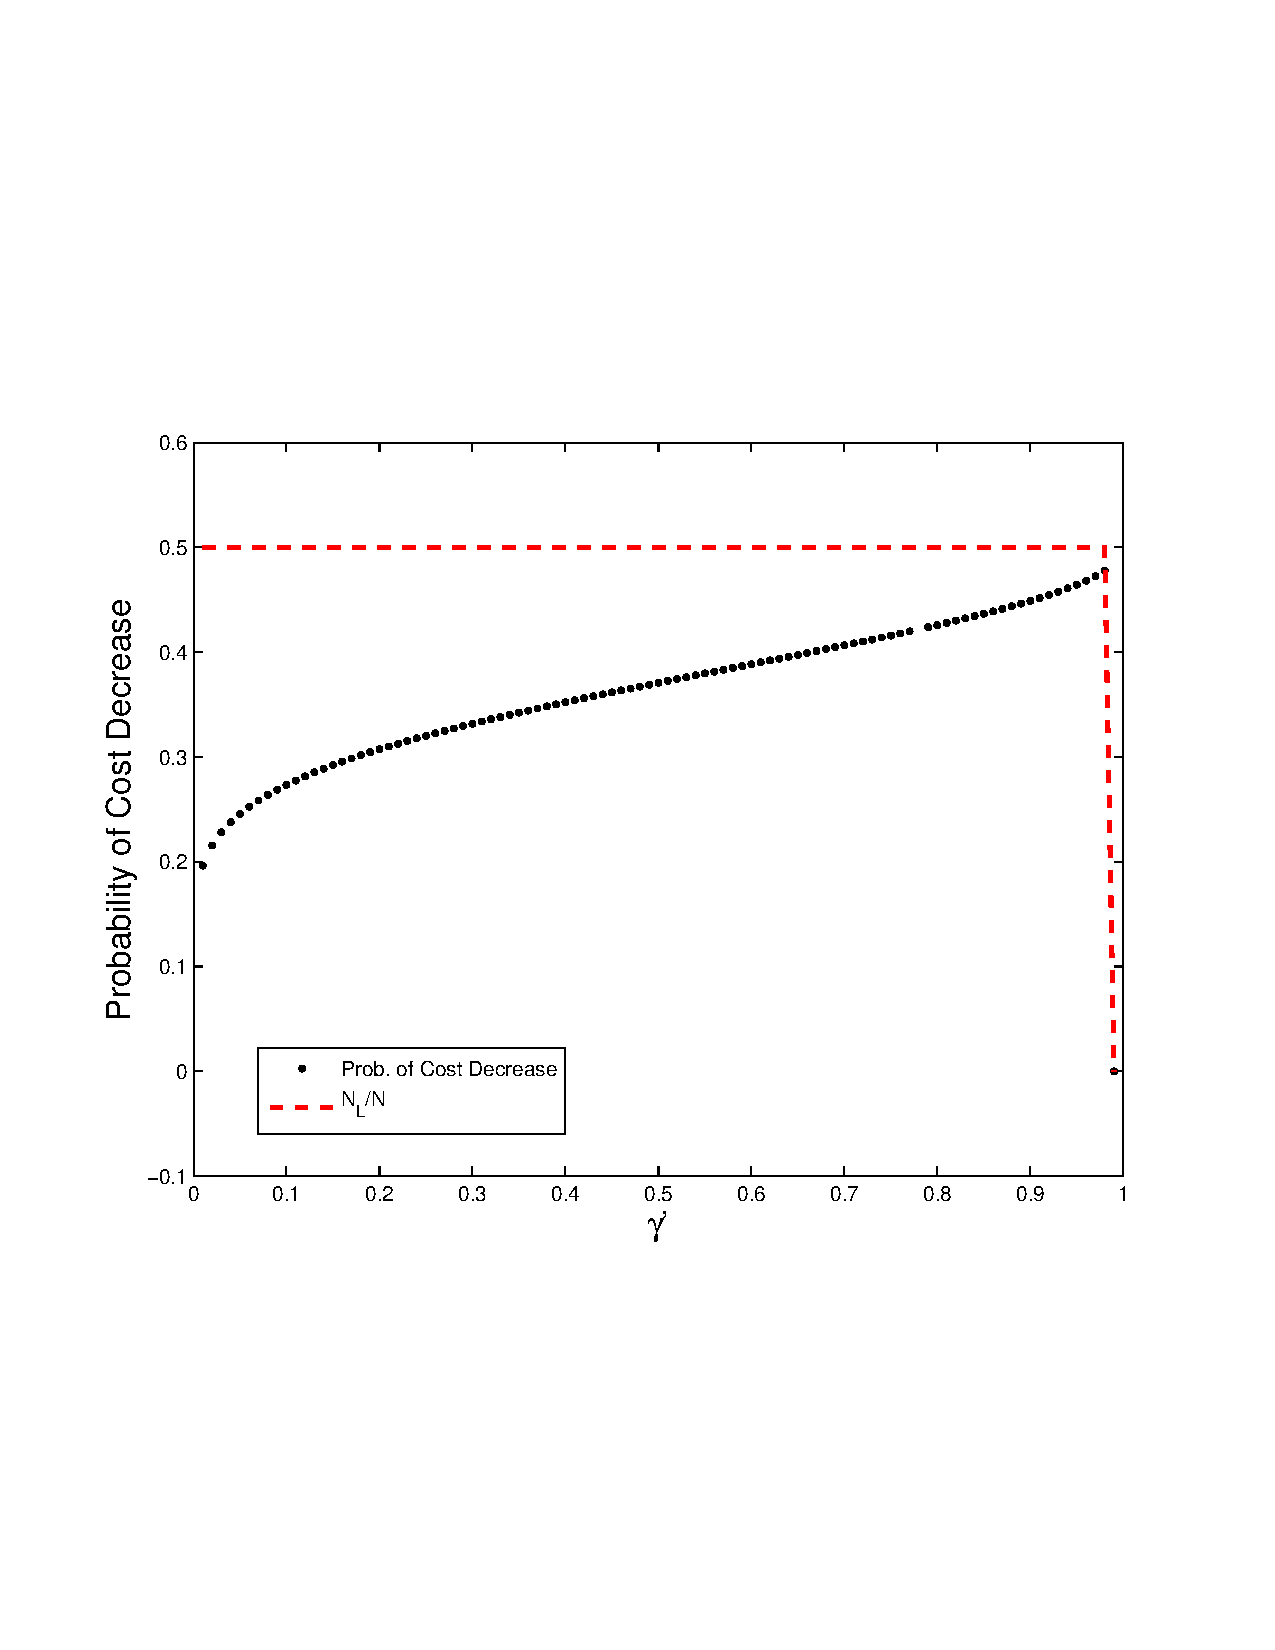
\includegraphics[width=.5\textwidth]{images/water_prob_decrease}
% 	\caption{Probability that an additional sample causes a decrease in worst-case expected cost for the likelihood robust water allocation problem.  The red line shows the upper bound probability $\tfrac{N_L}{N}$.}
% 	\label{fig:water_prob_decrease}
% \end{figure}

%%%%%%%%%%%%%%%%%%%%%%%%%%%%%%%%%%%%%%%%%%%%%%%%%%%%%%%%%%%%%%%%%%%%%%%%%%%%%%%%
\section{Summary and Future Work}
\label{sec:concl}

We proposed to use $\phi$-divergences
% constrained distributionally robust optimization method of \cite{bental2011robust} for two-stage stochastic linear programs with recourse, creating a two-stage $\phi$-divergence constrained ambiguous stochastic linear program with recourse, denoted \plp.
%The \plp\ uses a $\phi$-divergence 
to define an ambiguity set of probability distributions, possibly using observed data, and optimize the worst-case expected cost with respect to this ambiguity set in a two-stage setting.
We provided a new classification of $\phi$-divergences that can be used in determining which $\phi$-divergence is most appropriate in practice for different model types and decision makers.
A computationally simple method is established to determine if an additional sample %will produce a likelihood ambiguity set that does not contain the current worst-case distribution and
will result in a lower-cost solution.
We have shown that as more data is gathered, the optimal value and solution of \plp\ converge to those of SLP-2. 
We have also provided a Bender's decomposition-based solution algorithm to solve \plp\ efficiently and used it to illustrate some of the properties of the \plp.
% on a small electricity generation problem.

There are many interesting avenues for future work. 
One is the multi-stage extensions of the work provided here. 
Ways to handle continuous distributions in the \plp\ also merits further research. 
There are other divergences, probability metrics, and statistical ways to measure the distance between two distributions. 
Generalizations of the results presented in this paper to other distance measures is another area of future research. 
Finally, it would be useful to study applications to real-world problems.

% Acknowledgments here
% \ACKNOWLEDGMENT{%
% This work has been partially supported by the National Science Foundation through grant CMMI-1345626. We also gratefully acknowledge support provided by a Water Sustainability Program Fellowship through the Technology and Research Initiative Fund at the University of Arizona.
% }% Leave this (end of acknowledgment)


% Appendix here
% Options are (1) APPENDIX (with or without general title) or 
%             (2) APPENDICES (if it has more than one unrelated sections)
% Outcomment the appropriate case if necessary
%

\section*{Acknowledgements}
Support provided by a Water Sustainability Program Fellowship through the Technology and Research Initiative Fund at the University of Arizona.
This work has also been partially supported by the National Science Foundation through grant CMMI-1151226.

We acknowledge the World Climate Research Programme's Working Group on Coupled Modelling, which is responsible for CMIP, and we thank the climate modeling groups (listed in Table \ref{tb:climate_models} of this paper) for producing and making available their model output.
For CMIP the U.S. Department of Energy's Program for Climate Model Diagnosis and Intercomparison provides coordinating support and led development of software infrastructure in partnership with the Global Organization for Earth System Science Portals.

% References here (outcomment the appropriate case) 

% CASE 1: BiBTeX used to constantly update the references 
%   (while the paper is being written).
%\bibliographystyle{ijocv081} % outcomment this and next line in Case 1
\bibliography{love_lro} % if more than one, comma separated

% CASE 2: BiBTeX used to generate mypaper.bbl (to be further fine tuned)
%\input{mypaper.bbl} % outcomment this line in Case 2

%\section*{Author Biographies}

%\noindent {\bf DAVID LOVE} is a graduate student in the Graduate Interdisciplinary Program in Applied Mathematics at the University of Arizona.
%His research interests include distributionally robust stochastic programming and water resources management.
%His email address is \url{dlove@math.arizona.edu} and his web page is \url{http://math.arizona.edu/~dlove}.

%\bigskip

%\noindent {\bf G\"{U}ZIN BAYRAKSAN} is an Associate Professor of Integrated Systems Engineering at the Ohio State University.
%Her research interests include Monte Carlo sampling methods for stochastic programming and applications to water resources.
%Her email address is \url{bayraksan.1@osu.edu} and her web page is \url{http://www-iwse.eng.ohio-state.edu/biosketch_GBayraksan.cfm}

\end{document}

